\documentclass[12pt]{report}
\usepackage{%
	amsfonts,%
	amsmath,%	
	amssymb,%
	amsthm,%
	algorithm,%
%	babel,%
	bbm,%
	etex,%
	%biblatex,%
	caption,%
	centernot,%
	color,%
	dsfont,%
	enumerate,%
	epsfig,%
	epstopdf,%
	geometry,%
	graphicx,%
	hyperref,%
	latexsym,%
	mathtools,%
	multicol,%
	pgf,%
	pgfplots,%
	pgfplotstable,%
	pgfpages,%
	proof,%
	psfrag,%
	subfigure,%	
	tikz,%
	ulem,%
	url%
}
\usepackage{qtree}
\usepackage[fleqn]{amsmath}
\usepackage{amsthm}
\usepackage{csquotes} 
\usepackage[noend]{algpseudocode}
\usepackage[mathscr]{eucal}
\usepgflibrary{shapes}
\usetikzlibrary{%
  	arrows,%
	backgrounds,%
	chains,%
	decorations.pathmorphing,% /pgf/decoration/random steps | erste Graphik
	decorations.text,%
	matrix,%
  	positioning,% wg. " of "
  	fit,%
	patterns,%
  	petri,%
	plotmarks,%
  	scopes,%
	shadows,%
  	shapes.misc,% wg. rounded rectangle
  	shapes.arrows,%
	shapes.callouts,%
  	shapes%
}

\theoremstyle{plain}
\newtheorem{thm}{Theorem}[section]
\newtheorem{lem}[thm]{Lemma}
\newtheorem{prop}[thm]{Proposition}
\newtheorem{cor}[thm]{Corollary}

\theoremstyle{definition}
\newtheorem{defn}[thm]{Definition}
\newtheorem{conj}[thm]{Conjecture}
\newtheorem{exmp}[thm]{Example}
\newtheorem{assum}[thm]{Assumption}
\newtheorem{axiom}[thm]{Axiom}
\newtheorem{theorem}{Theorem}[section]
\newtheorem{corollary}{Corollary}[theorem]
\newtheorem{lemma}[theorem]{Lemma}



\theoremstyle{remark}
\newtheorem{rem}{Remark}
\newtheorem{note}{Note}
\newtheorem{fact}{Fact}

\newcommand{\norm}[1]{\left\lVert#1\right\rVert}
\newcommand{\indep}{\!\perp\!\!\!\perp}
\DeclarePairedDelimiter\abs{\lvert}{\rvert}%
\newcommand\numberthis{\addtocounter{equation}{1}\tag{\theequation}}
\newcommand{\tr}{\operatorname{tr}}
\newcommand{\R}{\mathbb{R}}
\newcommand{\N}{\mathbb{N}}
\newcommand{\E}{\mathbb{E}}
\newcommand{\Z}{\mathbb{Z}}
\newcommand{\B}{\mathscr{B}}
\newcommand{\C}{\mathcal{C}}
\newcommand{\T}{\mathscr{T}}
\newcommand{\F}{\mathcal{F}}
\newcommand{\G}{\mathcal{G}}
%\newcommand{\ba}{\begin{align*}}
%\newcommand{\ea}{\end{align*}}
\newcommand{\expect}[1]{\mathbb{E}\left[{#1}\right]}
\newcommand{\prob}[1]{\mathbb{P}\left[{#1}\right]}
\newcommand{\probo}[1]{\mathbb{P}_0\left[{#1}\right]}
\newcommand{\probi}[1]{\mathbb{P}_1\left[{#1}\right]}
\newcommand{\given}{\; \big\vert \;} 
\newcommand{\bydef}{:=}
\newcommand{\indic}[1]{\mathbbm{1}\{#1\}}
\DeclareMathOperator*{\argmax}{arg\,max}
\renewcommand{\qedsymbol}{$\blacksquare$}
\makeatletter
\def\BState{\State\hskip-\ALG@thistlm}
\makeatother

\makeatletter
\def\th@plain{%
  \thm@notefont{}% same as heading font
  \itshape % body font
}
\def\th@definition{%
  \thm@notefont{}% same as heading font
  \normalfont % body font
}
\makeatother
\date{}
\usepackage{scribe_e1244}
\usepackage{times}
\begin{document}
\lecturer{Aditya Gopalan}	% optional, put lecturer's name here
\scribe{Raseena KT, Shanuja Sasi}		% required, put your name here
\lecturenumber{4}			% required, must be a number
\lecturedate{January 12}		% required, omit year
\maketitle

% title of the lecture
\begin{center}
{\Large \bf Continuation of Minimax Hypothesis Testing}
\end{center}

% ----------------------------------------------------------------------


\section{Recap}

We assume that there are two possible hypotheses, $H_0$ and $H_1$, which correspond to two probability distributions $\mathbb{P}_0$ and $\mathbb{P}_1$, respectively, on $(\Gamma, \mathcal{G})$ where $\Gamma$ is the observation set and $\mathcal{G}$ is the class of subsets of $\Gamma$ that can be assigned probabilities. \\

\section{Minimax Hypothesis Testing}

The structure of minimax rules has already been stated in the lecture 3.
  
\noindent For case (3), i.e, for $\R_0$($\delta_{\pi_L}$) = $\R_1$($\delta_{\pi_L}$) , suppose v($\pi_0$) is differentiable at its maximum $\pi_L$.

\begin{eqnarray}
  \nonumber V(\pi_0) &\le& r(\pi_0, \delta_{\pi_L}) \hspace{0.5cm}\forall \hspace{0.25cm} \pi_0 \in [0,1], \\
    \nonumber  V(\pi_L) &=& r(\pi_L, \delta_{\pi_L}).
\end{eqnarray}


\noindent Therefore the line r( . ,$\delta_{\pi_L}$)  is tangent to V($\pi_0$) at $\pi_L$.If V($\pi_0$) is differentiable at $\pi_L \in$ (0,1).
\begin{align}
  \nonumber  0 &= V^\prime(\pi_L) \\\nonumber &= \frac{d}{{d\pi_0 }}V(\pi_0)\left| {_{\pi_0  = {\pi _L}}} \right.\\\nonumber  &= \frac{d}{{d\pi_0 }}r(\pi_0 {\delta _{{\pi _L}}})\left| {_{\pi_0  = {\pi _L}}} \right.\\\nonumber
&= {R_0}({\delta_{{\pi_L}}})- {R_1}({\delta_{{\pi_L}}})
\end{align} 
which implies
\begin{equation}
 \nonumber {R_0}({\delta_{{\pi_L}}})={R_1}({\delta_{{\pi_L}}}).
\end{equation}

In all the above Minimax Hypothesis testing approach we have assumed that the function $V(\pi_0)$ is continuous at the point of maxima.This may not be the case in many problems of interest. From the below tree structure , it can be seen that minimax rules are designed for all the cases except when the function V is not differentiable at its maximum interior point $\pi_L$.\\

\Tree[.$\pi_L\textit{:Maximizer of V}$  [.$\pi_L$\in\{0,1\} \textit{$\delta_{\pi_{L}}$is the minimax rule} ]
               [.$\pi _L$\in (0,1) [.\textit{V is differentiable at $\pi_L$} \textit{$\delta_{\pi_L}$ is the minimax rule} ]
                                      [.\textit{V is not differentiable at $\pi_L$ } \textit{?} ]]]\\\\
 \begin{exmp}
 Consider the binary channel hypothesis testing discussed in lecture 2. The observation space $\Gamma$ contains only two elements 0 and 1. Therefore there are only four possible decision rules namely $\delta_1,\delta_2,\delta_3$ and $\delta_4$. It is illustrated in the figure 4.2. It can be seen that the function V  is not differentiable at its maxima $\pi_L$. In  cases like this a randomized decision rule $\delta ^\ast$ solves the minimax problem.
   \end{exmp}
\begin{figure}[H]
  \centering
    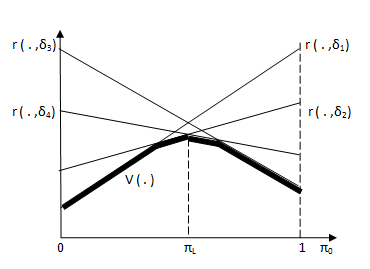
\includegraphics[height= 10cm, width=12cm]{Figures/Lec4_Fig1.PNG}
    \caption[]{Binary channel hypothesis testing}
\end{figure}


\begin{defn}
\textbf{Randomized decision rule} \nonumber  $\delta ^\ast$ maps  $\Gamma \to [0, 1]$. 
\begin{align}
 \nonumber  \delta ^\ast: \Gamma \to [0, 1]
\end{align}
\end{defn}

\noindent\textit{Interpretation}:After having seen y $\in \Gamma$, the rule decides $H_1$ with probability $\delta$(y) and $H_0$ with probability 1 - $\delta$(y).
\begin{assum}
Assume $C_{11}-C_{01} <$ 0 and $C_{00}-C_{10} <$ 0 without loss of generality.
\end{assum}
\noindent For any $\pi_0 < \pi_L$, the bayes rule is
\begin{equation}
\Gamma_1(\delta_{\pi_0}) = \{y\in\Gamma:L(y)\ge\tau (\pi_0)\}, \nonumber \end{equation}
where
\begin{equation}
 \nonumber \tau (\pi_0)=\frac{\pi_0(C_{00}-C_{10} )}{(1-\pi_0)(C_{11}-C_{01})}
\end{equation}
$\tau(\pi_0)$ is a monotonically increasing function of $\pi_0$. And hence $\forall \hspace{0.1cm} \pi_0^\prime <\pi_0^{\prime\prime}<\pi_L$, we have\\
\begin{align}
 \nonumber \Gamma_1(\delta_{\pi_0^{\prime}}) \subseteq\Gamma_1(\delta_{\pi_0^{\prime\prime}})
\end{align}
\begin{eqnarray}
 \text{Define:} \hspace{2cm} 
\nonumber \Gamma_{1}^{-} &=& \underset{\pi_0 < \pi_L}{\bigcap} \{ \Gamma_{1}(\delta_{\pi_{0}^{\prime}})\} \\\nonumber &=& \underset{\pi_0 < \pi_L}{\bigcap} \{ L(y) \geq \tau(\pi_0)\} \\ &=& \{ y \in \Gamma : L(y) \geq \tau(\pi_L) \}.  \\
\nonumber \Gamma_{1}^{+}  &=& \underset{\pi_0 < \pi_L}{\bigcup} \{ \Gamma_{1}(\delta_{\pi_{0}^{\prime}})\} \\ \nonumber &=& \underset{\pi_0 < \pi_L}{\bigcup} \{ L(y) > \tau(\pi_0)\}\\ &=& \{ y \in \Gamma : L(y) > \tau (\pi_L) \}.
\end{eqnarray}

\noindent The difference in the inequalities of the equations (4.15) and (4.16) is due to the following reason:
\begin{align}
\underset{\pi_0 <0}{\bigcap}[\pi_0,\infty)=[0,\infty)=\{y:y\ge0\},\\
\underset{\pi_0 >0}{\bigcup}[\pi_0,\infty)=(0,\infty)=\{y:y<0\}.
 \end{align}
 \noindent Equation (4.17) is similar to (4.15) and  (4.18) is similar to (4.16) and hence the difference in the inequalities arises.\\ \\
From the equations (4.15) and (4.16)
\begin{align}
 \nonumber {\Gamma_{1}^{-}}\supseteq{\Gamma_{1}^{+}}
\end{align}}
which implies,
\begin{align}
 \nonumber {\Gamma_{1}^{-}}^{c}\subseteq{\Gamma_{1}^{+}}^{c}
\end{align}
The observation space is illustrated in the figure 4.3.\\
\begin{figure}[H]
  \centering
    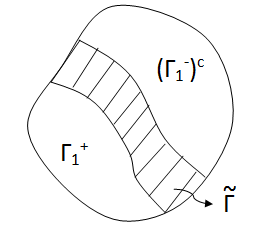
\includegraphics[height= 5cm, width=6cm]{Figures/Lec4_Fig2.PNG}    \caption[]{Division of the observation space $\Gamma$}
\end{figure}



\noindent Take some $q\in[0,1]$ and define the randomized rule $\delta_q$ as:



\begin{equation}
{{\delta}_{q}(y)}  = 
\begin{cases}
1, &\mbox{if }~y \in \Gamma_1^{+},\\
0, &\mbox{if }~y \in {(\Gamma_1^{-})}^c,\\
\begin{cases}
\text{1 with probability q} \\ \text{0 with probability 1-q }
\end{cases} &\mbox{if }~y \in \widetilde{\Gamma}.
\end{cases}
\end{equation}
Let $\delta^+$ be the decision rule that divides observation space $\Gamma$ into $\Gamma_1^{+}$ and $(\Gamma_1^{+})}^c$ and $\delta^-$ be the decision rule that divides observation space into $\Gamma_1^{-}$ and $(\Gamma_1^{-})}^c$ .\\ \\
\textit{Claim 1}: Bayes risk of $\delta_q$ = bayes risk of $ \delta^+$ = bayes risk of $\delta^-$.\\
\begin{proof}
This is because boundary decision is irrelevant to bayes risk.
\end{proof}
\noindent Since conditional risk depends on the boundary condition, it can be written as,
\begin{align}
R_j(\delta_{q}) &= qR_j(\delta^{-}) + (1-q)R_j(\delta^{+}), \hspace{0.75cm}j \in \{0,1\}
\end{align}
\noindent which is nothing but, 
\begin{align}
R_0({{\delta}_{q}}) &= qR_0(\delta^{-}) + (1-q)R_0(\delta^{+}), \nonumber \\
 \nonumber R_1({{\delta}_{q}}) &= qR_1(\delta^{-}) + (1-q)R_1(\delta^{+}). 
\end{align}
So for the minimax rule at equality,
\begin{equation}
\max\{ R_0({{\delta}_{q}}), R_1({{ \delta}_{q}}) \} = R_0({{ \delta}_{q}}) = R_1({{ \delta}_{q}}).
\end{equation}
Therefore, the conditional risk equations for equality condition are,
\[
\begin{array}{@{}l@{}} 
\nonumber qR_0(\delta^{-}) + (1-q)R_0(\delta^{+})=qR_1(\delta^{-}) + (1-q)R_1(\delta^{+}),\\
\nonumber q\{R_0(\delta^{-}) - R_0(\delta^{+})\} + R_0(\delta^{+})= q\{R_1(\delta^{-}) - R_1(\delta^{+})\} + R_1(\delta^{+}),\\
\nonumber R_0(\delta^{+}) - R_1(\delta^{+}) = q\{R_0(\delta^{+}) - R_1(\delta^{+}) + R_1(\delta^{-}) - R_0(\delta^{-})\}.
\end{array}
\]
So,
\begin{equation}
\label{qeq}
q = \frac{R_0(\delta^{+}) - R_1(\delta^{+})}{R_0(\delta^{+}) - R_1(\delta^{+}) + R_1(\delta^{-}) - R_0(\delta^{-})}.
\end{equation}
This gives the probability with which we choose the alternate hypothesis at the boundary, which is equivalent to throwing a biased coin with probability $q$ and
selecting a decision rule based on the outcome.
\begin{rem}
We now represent the unconditional risk by $V$. Since $V$ is concave, it must have left hand and right hand derivative at $\pi_L$, which is denoted by $V^{'}(\pi_L^{-})$ and $V^{'}(\pi_L^{+})$. Now,
\begin{eqnarray}
V^{'}(\pi_L^{-}) &=& \frac{d}{d \pi_0} r(\pi_0 , \delta_{\pi_L}^{-})\nonumber \\
&=& \frac{d}{d\pi_0}\{\pi_0 R_0(\delta_{\pi_L}^{-}) + (1-\pi_0)R_1(\delta_{\pi_L}^{-}) \}\nonumber \\
&=& R_0(\delta_{\pi_L}^{-}) - R_1(\delta_{\pi_L}^{-}). 
\end{eqnarray}
Similarly,\hspace{2.5cm}$V^{'}(\pi_L^{+}) = R_0(\delta_{\pi_L}^{+}) - R_1(\delta_{\pi_L}^{+})$. \\Hence eqn. (\ref{qeq}) can be written as
\begin{equation}
q = \frac{V^{'}(\pi_L^{+})}{V^{'}(\pi_L^{+}) - V^{'}(\pi_L^{-})}.
\end{equation}
\end{rem}
We can analyze the importance of the above equation in the following manner. Figure \ref{fig:DecisionRules} shows the case in which $V$ is discontinuous at the point of maxima. The decision rule here is ${{ \delta}_{q}}$. By varying the probability $q$ from $0$ to $1$, different slopes of the line $r(\pi_0, {{\delta}_{\pi_L}})$ can be obtained. The particular value $q$ obtained from the equation above corresponds to the horizontal line.   
\begin{figure}[h]
\centering
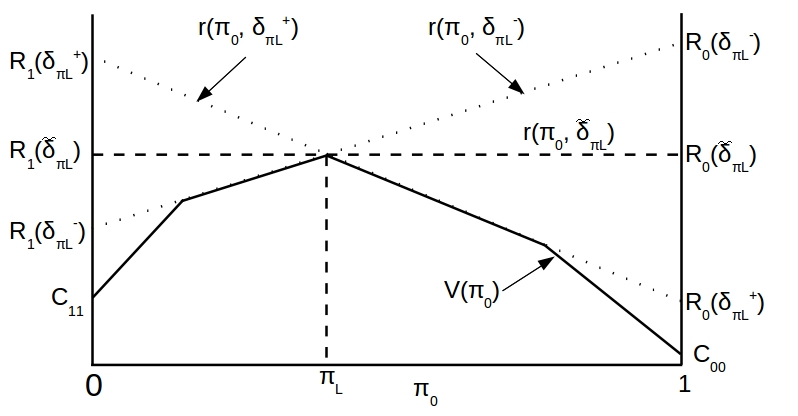
\includegraphics[width=0.7\linewidth]{Figures/Lec4_Fig3.jpg}
\caption[rdr]{Action of the randomized decision rule}
\label{fig:DecisionRules}
\end{figure}
\newpage
\noindent Hence we can complete the tree structure as below:\\

\Tree[.$\pi_L\textit{:Maximizer of V}$  [.$\pi_L$\in\{0,1\} \textit{$\delta_{\pi_{L}}$is minimax rule} ]
               [.$\pi _L$\in (0,1) [.\textit{V is differentiable at $\pi_L$} \textit{$\delta_{\pi_L}$ is minimax rule} ]
                                      [.\textit{V is not differentiable at $\pi_L$ } \textit{$\delta_{q}$ is the minimax rule} ]]]


\begin{exmp}[Location testing with Gaussian error]The input to the channel is real numbers.Here there are two possible inputs $\mu_0$ and $\mu_1$. The gaussian noise is added to the input and the output is produced. The goal here is to guess which of $\mu_0$ or $\mu_1$ was sent.


\begin{figure}[h]
\centering
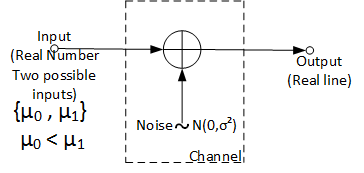
\includegraphics[scale=1]{Figures/Lec4_Fig4}
\caption{Location Testing with Gaussian Error.}
\label{fig:LocationTest}
\end{figure}
\begin{align*}
\Gamma &\bydef \Re\\
H_j &= \mu_j \in \Re \text{ is the input, $j \in \{0,1\}$}\\
\mathbbm{P}_j &= N(\mu_j,\sigma^2), j \in \{0,1\}
\end{align*}
\newpage
\noindent Consider the case of uniform costs, i.e, $\C_{ij} = \indic{i \neq j}$

\begin{equation}
   \nonumber   V(\pi_0) = \pi_0 R_0(\delta_{\pi_0}) + \pi_1 R_1(\delta_{\pi_0})
\end{equation}
\noindent $\delta_{\pi_0}$ has the form:
\begin{align*}
\Gamma_1 &= \{ y \in R : L(y) \geq \tau (\pi_0)\} \\
&= \{ y : y \geq \tau^\prime\}.\\
\end{align*}
 
\noindent where L(y)=$\frac{p_1(y)}{p_0(y)}$ , \\
$p_1(y)$ :Probability that y is produced by hypothesis 1\\
$p_0(y)$ :Probability that y is produced by hypothesis 0
\\ \\
\noindent From the example 2.2.2 from lecture 2,
\begin{align}
 \nonumber  \tau^\prime = \frac {\mu_0+\mu_1}{2}+\frac{{\sigma}^2 \ln\tau}{\mu_1-\mu_0}
\end{align}
\begin{eqnarray}
   \nonumber   V(\pi_0)\nonumber &=&\pi_0 \int_{\tau^\prime}^{\infty} P_0(y) \,dy + (1 - \pi_0) \int_{-\infty}^{\tau^\prime} P_1(y) \,dy \\
&=& \pi_0 [1 - \phi(\frac{\tau^\prime - \mu_0}{\sigma})] + (1 - \pi_0) \phi(\frac{\tau^\prime - \mu_1}{\sigma}).
\end{eqnarray}

\noindent $\phi$ is the CDF (Cumulative Distribution Function) of standard normal random variable.\\
It turns out that V($\pi_0$) is maximized at $\pi_0$= $\frac{1}{2}$.So the minimax rule is simply $\delta_{\frac{1}{2}}$. i.e,
\begin{equation}
  \nonumber    \delta_{\frac{1}{2}} = \indic{ y \geq \frac {\mu_0+\mu_1}{2} }.
\end{equation}

\end{exmp}

\bibliography{Lecture_04_Scribe_Notes}
\bibliographystyle{IEEEtran}
\end{document}